
\documentclass[10pt]{article}

\linespread{1} 
\usepackage{float}

\usepackage{geometry}
 \geometry{
  papersize={175mm,248mm},
 total={175mm,248mm},
 left=26mm,
 right=13mm,
 bottom=17mm,
 top=13mm,
 }


\usepackage{amsfonts,amssymb,graphicx,color,epstopdf}
\usepackage[font=small,labelfont=bf]{caption}
\usepackage{subcaption}

\usepackage{color, colortbl, framed}
\usepackage[T1]{fontenc}
\usepackage{mathptmx}

\usepackage{amsmath}
%\usepackage{lineno,hyperref}
\usepackage{authblk}
\usepackage{titlesec}
\usepackage{eucal}
%\DeclareMathAlphabet{\mathpzc}{OT1}{pzc}{m}{it}
%\usepackage{epstopdf}

\usepackage{hhline}
\usepackage{xcolor,colortbl}
\renewcommand{\figurename}{Fig.}

%  \setcounter{secnumdepth}{0}
\usepackage{titlesec}
\titlespacing{\section}{0pt}{\parskip}{-\parskip}
\titlespacing{\subsection}{0pt}{\parskip}{-\parskip}
 \titleformat*{\section}{\normalfont\fontfamily{ptm}\fontsize{10}{19}\bfseries}
 \titleformat*{\subsection}{\normalfont\fontfamily{ptm}\fontsize{10}{18}\bfseries}


\usepackage[sort&compress,square]{natbib}
\setlength{\bibsep}{0.0pt}


\usepackage{authblk}
\usepackage{varwidth}

\renewcommand*{\Authsep}{, }
\renewcommand*{\Authand}{, }
\renewcommand*{\Authands}{, }
\renewcommand*{\Affilfont}{\normalsize\normalfont}
\renewcommand*{\Authfont}{\normalsize\normalfont\bfseries}
\setlength{\affilsep}{0em}

\renewcommand{\abstractname}{}    % clear the title
\makeatletter
\renewcommand{\maketitle}{\bgroup\setlength{\parindent}{0pt}
\begin{flushleft}
  \textbf{\@title}
\vspace{10pt}

  \@author
\end{flushleft}\egroup
}
\makeatother

\title{\fontsize{16pt}{10pt}\selectfont\flushleft \textbf{Application of principal component analysis of time-frequency representation for gearbox fault detection}}

\author[1]{Jacek Wodecki}
% \cortext[cor1]{Corresponding author, jacek.wodecki@pwr.edu.pl}
\author[1]{Justyna Hebda-Sobkowicz}
\author[2]{Agnieszka Wy{\l}oma{\'n}ska}
\author[1]{Radoslaw Zimoz}
\author[3,4]{Konstantinos Gryllias}


\affil[1]{Diagnostics and Vibro-Acoustic Science Laboratory, Wroclaw University of Science and Technology, Na Grobli 15, 50-421 Wroclaw}
\affil[2]{KGHM Cuprum Ltd, Research and Development Centre, Sikorskiego 2-8, 53-659 Wroclaw, Poland}
\affil[3]{Department of Mechanical Engineering, KU Leuven, Celestijnenlaan 300 - box 2420, 3001 Leuven, Belgium}
\affil[4]{Core Lab Dynamics of Mechanical and Mechatronic Systems, Flanders Make, Belgium
\protect\\
\textbf{E-mail:} $^{1}${\{jacek.wodecki, justyna.hebda-sobkowicz, radoslaw.zimroz\}@pwr.edu.pl}, $^{2}${awylomanska@cuprum.wroc.pl}, $^{3, 4}${konstantinos.gryllias@kuleuven.be}}


\date{} 

\begin{document}
\maketitle
\textbf{Abstract.} Dimensionality reduction methods are very useful and effective tools in the field of data analytics, used either independently or as a pre-processing step in the frames of a complex algorithm. In this paper a simple yet powerful technique for local damage detection in heavy-duty industrial machinery is presented with particular focus on gearboxes. It assumes that the cyclic component present in the vibration signal carrying information about the damage, can be extracted from relevant frequency bands of the signal. Although this assumption is usually a starting point for selective filtration in the notion of Informative Frequency Band (IFB) identification, in this case the frequency bands are not addressed directly. The authors propose to apply Principal Component Analysis (PCA) as a dimensionality reduction method on the time-frequency representation of the input data in such a way, that the dimension of frequency is reduced. In this way, the variance maximized in the first principal component is expected to capture the cyclic information which is related to the damage present in the machine.
\newline \newline
\textbf{Keywords:} Local damage detection, Vibrations, Principal Component Analysis, Time-Frequency analysis.

\section{Introduction}

The topic of fault detection in rotating machines is still an open problem in the field of machine diagnostics. Several reviews on damage detection in bearings and gears can be found in literature \cite{randall2011rolling,samuel2005review,feng2013recent}. The yypical methods take advantage of Higher-Order Statistics \cite{antoni2006spectral}, the Wavelet Transform \cite{lin2003gearbox}, the Time-Frequency domain analysis \cite{burdzik2014structural,feng2013recent}, the Bi-frequency analysis \cite{borghesani2014relationship} etc. The Vibration signals capture on a machinery system are often a mixture of several source signals. For instance, a signal acquired on a bearing operating in a belt conveyor driving station might be contaminated with vibrations from a neighboring gearbox or by vibrations caused by other damage. Another example is the analysis of a multi-source signal that is acquired on a gearbox with two faults, each of different nature \cite{zak2014novel}. In this paper PCA is used for local damage detection in a two-stage gearbox operating in a belt conveyor driving station. The PCA is applied on the Short-Time Fourier Transform (STFT) of the measured vibration signal in order to reduce its dimensionality, which is a common method for this purpose \cite{bartkowiak2014dimensionality,bartkowiak2012data}. The authors propose to focus on the analysis of the first principal component produced by the PCA algorithm. The method allows to discover the waveform that represents the fault component within the overall vibration data.

\section{Methodology}
Firstly, the signal has to be transformed into a time-frequency domain. For such transformation, the spectrogram has been chosen. The Short-time Fourier transform is given for discrete data $x[0], x[1], ... , x[N-1]$ by the formula \cite{allen1977short}:
\begin{equation}
    \textrm{STFT}(k,n)=\sum_{m=0}^{L-1}x[n+m]w[m]e^{-j2\pi km/N},
\end{equation}
where $0\leq k \leq N-1$ is the frequency bin, $n$ is the time point and  $w[\cdot]$ is the window of length $L$. One can observe that in the STFT for each time point the Fourier transform is calculated using the FFT algorithm. Furthermore, the spectrogram is equal to the squared absolute value of the STFT:

\begin{equation}
\textrm{Spec}(k,n)=|\textrm{STFT}(k,n)|^2.
\end{equation}

In the next step the dimensionality of the obtained spectrogram matrix is reduced using principal component analysis with respect to frequency, so that the output contains vectors in time domain. 
\begin{figure}[ht!]
\centering
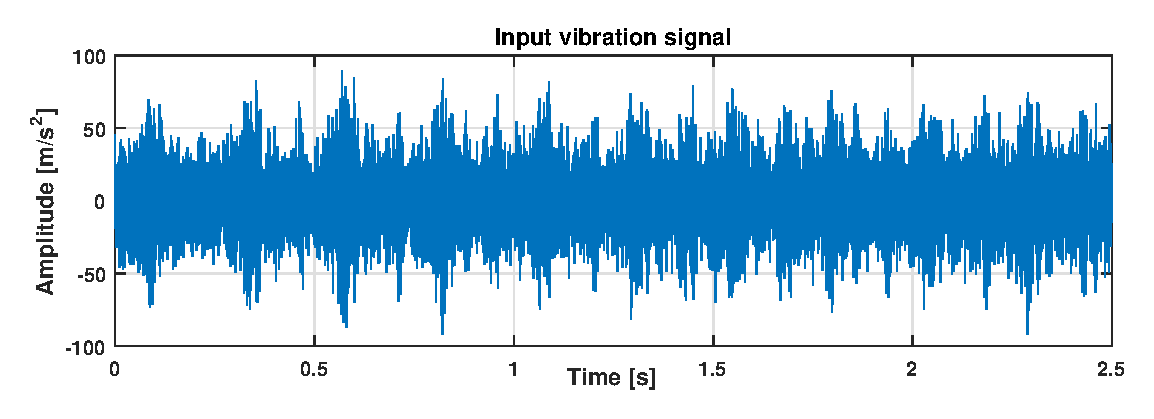
\includegraphics[width=0.8\textwidth]{wykresy/raw.eps}
\caption{Raw input signal}
\label{fig:raw}
\end{figure}
Principal component analysis is one of the most common and widespread methods for multivariate linear data analysis. It serves for investigating data structure, data mining, data smoothing and approximation as well as for exploring data dimensionality. The method permits to build new features, called Principal Components (PCs), which may serve for visualization of the data \cite{moore1981principal,wodecki2016combination,bartkowiak2014dimensionality,bartkowiak2012data}. 

\begin{figure}[ht!]
\centering
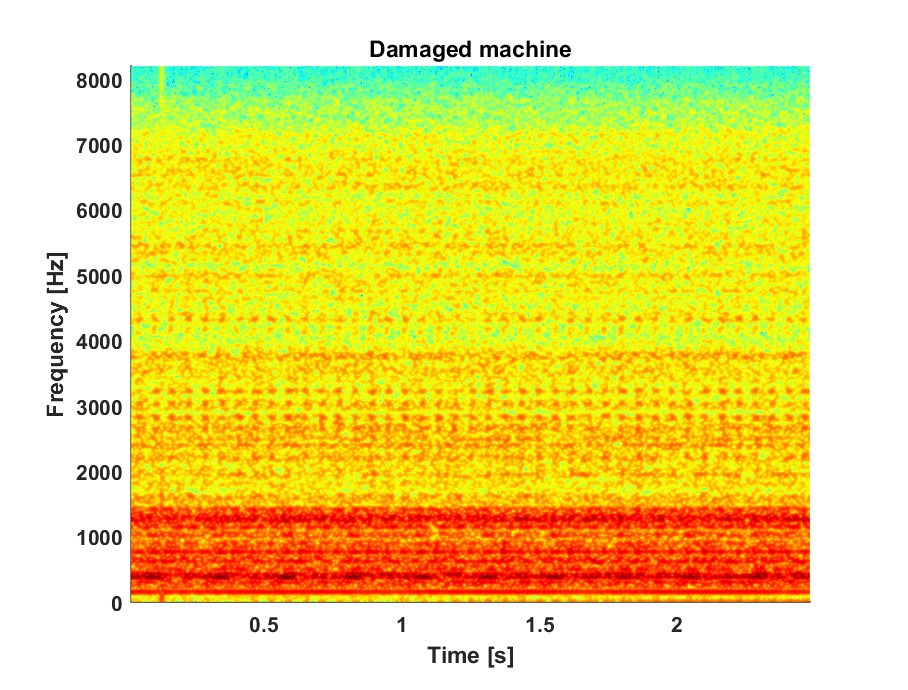
\includegraphics[width=0.7\textwidth]{wykresy/spec.eps}
\caption{Spectrogram of the input signal}
\label{fig:spec}
\end{figure}

Finally, the first PC is expected to capture the time-domain waveform of the damage component hidden in the signal.

\section{Application to industrial data}

The vector of observation contains a vibration signal of a two-stage gearbox in a belt conveyor driving station, commonly used in mining industry for material transportation (see Figure \ref{fig:raw}). The parameters of the data acquisition are selected as follows: duration 2.5 s, sampling frequency 16384 Hz and the expected fault frequency is equal to 16.5 Hz. Preliminary observations of the raw signal allow to observe a clearly visible amplitude modulation that is not related to the local damage under investigation but is related to a misalignment of the neighboring shaft. In order to decompose the process into more informative sub-processes the STFT has been applied. Hence the time-frequency spectrogram matrix, presented in Figure \ref{fig:spec}, is obtained.
% \begin{figure}[ht!]
% \centering
% 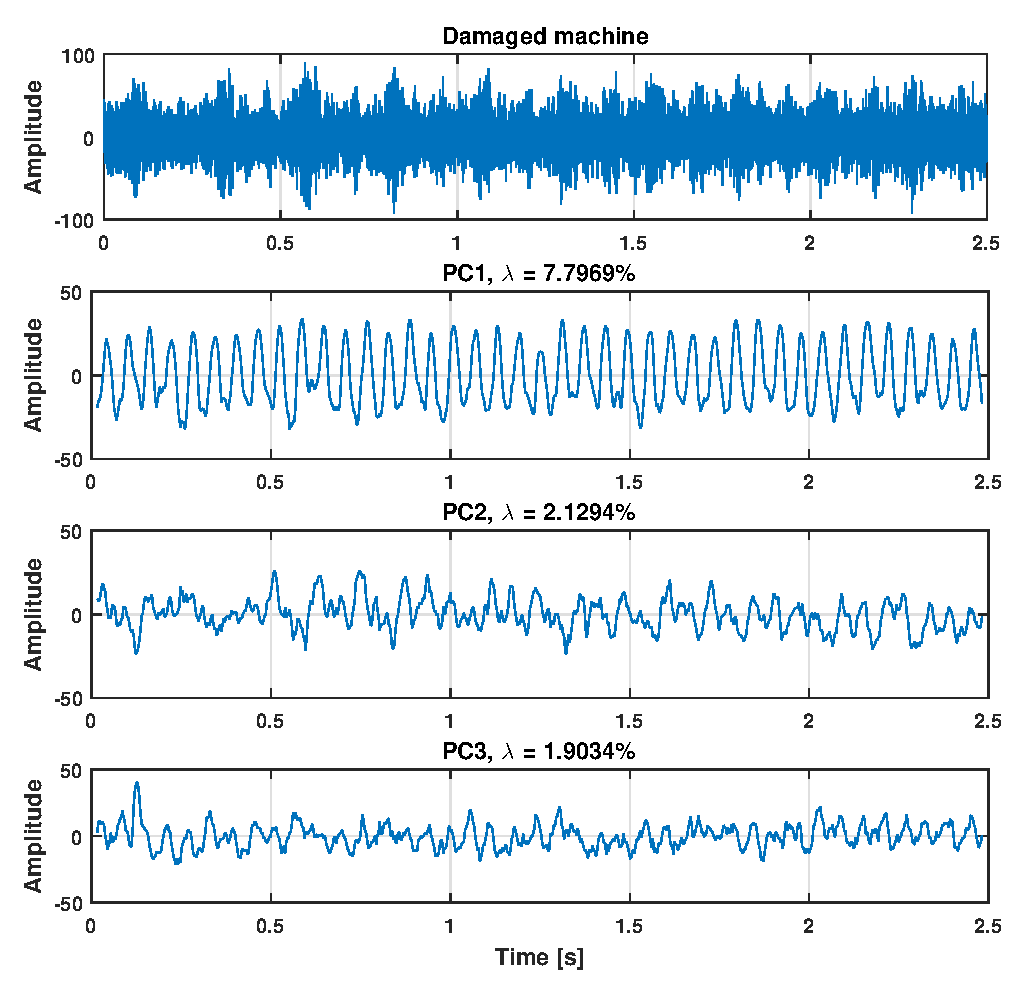
\includegraphics[width=0.7\textwidth]{wykresy/ts.eps}
% \caption{Raw signal with three first principal components}
% \label{fig:ts}
% \end{figure}
\begin{figure}[ht!]
\centering
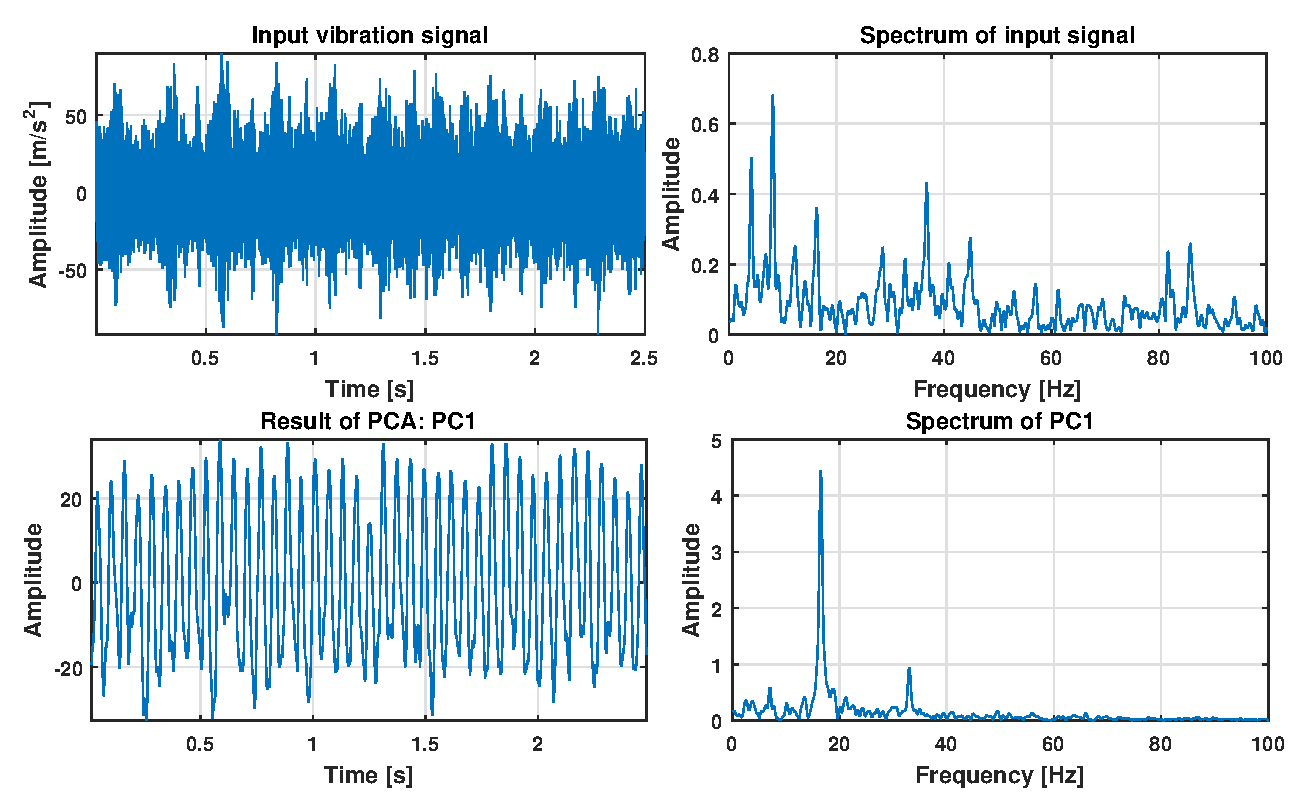
\includegraphics[width=\textwidth]{wykresy/widma.eps}
\caption{Fourier spectra of raw signal and first three components}
\label{fig:widmo}
\end{figure}
In the spectrogram one can observe three main frequency bands: a first one containing a low frequency with high energy responsible for the shape of the signal set at 0-1.5 kHz, a second one which contains two Informing Frequency Bands (IFB) placed at 2.5-3.5 kHz and 4-4,5 kHz and a third non-informative high frequency band above 5.3 kHz. PCA is applied on the spectrogram matrix and the first principal component is investigated and plotted in Figure \ref{fig:widmo} along with the original time series. The extracted principal component contains by definition the most relevant information content of the data. The remaining PCs have been omitted at this work.

The first principal component maximizes the variance, namely it takes into account as much of the variability in the data as possible and therefore the PC1 is treated as the component which is responsible for the fault description. The spectral signatures of the observed PC1 have been investigated in Figure \ref{fig:widmo}. As it was expected, the amplitude spectrum graph of PC1 gives very precise information about the fundamental frequency of the damage, equal to 16.5 Hz.



\section{Conclusions}
In this article, the authors proposed a simple yet robust approach to the detection of periodically impulsive behaviors in the vibration signal. This behavior is associated with a component with information about the fault. The analyzed data have been acquired from a two-stage gearbox of a complex mechanical system working in mining environment. In order to detect the frequency of the component which has been damaged, principal component analysis has been applied, using a time-frequency representation of the vibration data as the basis for the analysis. As a result, a clear and precise periodical component has been obtained, that can indicate the fault frequency, which is confirmed by the spectrum of the result component. Such information can be further used in identifying the faulty component in the process of the machine maintenance.
\section*{Acknowledgments}
The work of J.Wodecki and J.Hebda-Sobkowicz was supported by the statutory grant.
\bibliographystyle{style}
\bibliography{mybibfile}

\end{document}